%
\documentclass{article} % For LaTeX2e
\usepackage{iclr2021_conference,times}

% Optional math commands from https://github.com/goodfeli/dlbook_notation.
%%%%% NEW MATH DEFINITIONS %%%%%

\usepackage{amsmath,amsfonts,bm}

% Mark sections of captions for referring to divisions of figures
\newcommand{\figleft}{{\em (Left)}}
\newcommand{\figcenter}{{\em (Center)}}
\newcommand{\figright}{{\em (Right)}}
\newcommand{\figtop}{{\em (Top)}}
\newcommand{\figbottom}{{\em (Bottom)}}
\newcommand{\captiona}{{\em (a)}}
\newcommand{\captionb}{{\em (b)}}
\newcommand{\captionc}{{\em (c)}}
\newcommand{\captiond}{{\em (d)}}

% Highlight a newly defined term
\newcommand{\newterm}[1]{{\bf #1}}


% Figure reference, lower-case.
\def\figref#1{figure~\ref{#1}}
% Figure reference, capital. For start of sentence
\def\Figref#1{Figure~\ref{#1}}
\def\twofigref#1#2{figures \ref{#1} and \ref{#2}}
\def\quadfigref#1#2#3#4{figures \ref{#1}, \ref{#2}, \ref{#3} and \ref{#4}}
% Section reference, lower-case.
\def\secref#1{section~\ref{#1}}
% Section reference, capital.
\def\Secref#1{Section~\ref{#1}}
% Reference to two sections.
\def\twosecrefs#1#2{sections \ref{#1} and \ref{#2}}
% Reference to three sections.
\def\secrefs#1#2#3{sections \ref{#1}, \ref{#2} and \ref{#3}}
% Reference to an equation, lower-case.
\def\eqref#1{equation~\ref{#1}}
% Reference to an equation, upper case
\def\Eqref#1{Equation~\ref{#1}}
% A raw reference to an equation---avoid using if possible
\def\plaineqref#1{\ref{#1}}
% Reference to a chapter, lower-case.
\def\chapref#1{chapter~\ref{#1}}
% Reference to an equation, upper case.
\def\Chapref#1{Chapter~\ref{#1}}
% Reference to a range of chapters
\def\rangechapref#1#2{chapters\ref{#1}--\ref{#2}}
% Reference to an algorithm, lower-case.
\def\algref#1{algorithm~\ref{#1}}
% Reference to an algorithm, upper case.
\def\Algref#1{Algorithm~\ref{#1}}
\def\twoalgref#1#2{algorithms \ref{#1} and \ref{#2}}
\def\Twoalgref#1#2{Algorithms \ref{#1} and \ref{#2}}
% Reference to a part, lower case
\def\partref#1{part~\ref{#1}}
% Reference to a part, upper case
\def\Partref#1{Part~\ref{#1}}
\def\twopartref#1#2{parts \ref{#1} and \ref{#2}}

\def\ceil#1{\lceil #1 \rceil}
\def\floor#1{\lfloor #1 \rfloor}
\def\1{\bm{1}}
\newcommand{\train}{\mathcal{D}}
\newcommand{\valid}{\mathcal{D_{\mathrm{valid}}}}
\newcommand{\test}{\mathcal{D_{\mathrm{test}}}}

\def\eps{{\epsilon}}


% Random variables
\def\reta{{\textnormal{$\eta$}}}
\def\ra{{\textnormal{a}}}
\def\rb{{\textnormal{b}}}
\def\rc{{\textnormal{c}}}
\def\rd{{\textnormal{d}}}
\def\re{{\textnormal{e}}}
\def\rf{{\textnormal{f}}}
\def\rg{{\textnormal{g}}}
\def\rh{{\textnormal{h}}}
\def\ri{{\textnormal{i}}}
\def\rj{{\textnormal{j}}}
\def\rk{{\textnormal{k}}}
\def\rl{{\textnormal{l}}}
% rm is already a command, just don't name any random variables m
\def\rn{{\textnormal{n}}}
\def\ro{{\textnormal{o}}}
\def\rp{{\textnormal{p}}}
\def\rq{{\textnormal{q}}}
\def\rr{{\textnormal{r}}}
\def\rs{{\textnormal{s}}}
\def\rt{{\textnormal{t}}}
\def\ru{{\textnormal{u}}}
\def\rv{{\textnormal{v}}}
\def\rw{{\textnormal{w}}}
\def\rx{{\textnormal{x}}}
\def\ry{{\textnormal{y}}}
\def\rz{{\textnormal{z}}}

% Random vectors
\def\rvepsilon{{\mathbf{\epsilon}}}
\def\rvtheta{{\mathbf{\theta}}}
\def\rva{{\mathbf{a}}}
\def\rvb{{\mathbf{b}}}
\def\rvc{{\mathbf{c}}}
\def\rvd{{\mathbf{d}}}
\def\rve{{\mathbf{e}}}
\def\rvf{{\mathbf{f}}}
\def\rvg{{\mathbf{g}}}
\def\rvh{{\mathbf{h}}}
\def\rvu{{\mathbf{i}}}
\def\rvj{{\mathbf{j}}}
\def\rvk{{\mathbf{k}}}
\def\rvl{{\mathbf{l}}}
\def\rvm{{\mathbf{m}}}
\def\rvn{{\mathbf{n}}}
\def\rvo{{\mathbf{o}}}
\def\rvp{{\mathbf{p}}}
\def\rvq{{\mathbf{q}}}
\def\rvr{{\mathbf{r}}}
\def\rvs{{\mathbf{s}}}
\def\rvt{{\mathbf{t}}}
\def\rvu{{\mathbf{u}}}
\def\rvv{{\mathbf{v}}}
\def\rvw{{\mathbf{w}}}
\def\rvx{{\mathbf{x}}}
\def\rvy{{\mathbf{y}}}
\def\rvz{{\mathbf{z}}}

% Elements of random vectors
\def\erva{{\textnormal{a}}}
\def\ervb{{\textnormal{b}}}
\def\ervc{{\textnormal{c}}}
\def\ervd{{\textnormal{d}}}
\def\erve{{\textnormal{e}}}
\def\ervf{{\textnormal{f}}}
\def\ervg{{\textnormal{g}}}
\def\ervh{{\textnormal{h}}}
\def\ervi{{\textnormal{i}}}
\def\ervj{{\textnormal{j}}}
\def\ervk{{\textnormal{k}}}
\def\ervl{{\textnormal{l}}}
\def\ervm{{\textnormal{m}}}
\def\ervn{{\textnormal{n}}}
\def\ervo{{\textnormal{o}}}
\def\ervp{{\textnormal{p}}}
\def\ervq{{\textnormal{q}}}
\def\ervr{{\textnormal{r}}}
\def\ervs{{\textnormal{s}}}
\def\ervt{{\textnormal{t}}}
\def\ervu{{\textnormal{u}}}
\def\ervv{{\textnormal{v}}}
\def\ervw{{\textnormal{w}}}
\def\ervx{{\textnormal{x}}}
\def\ervy{{\textnormal{y}}}
\def\ervz{{\textnormal{z}}}

% Random matrices
\def\rmA{{\mathbf{A}}}
\def\rmB{{\mathbf{B}}}
\def\rmC{{\mathbf{C}}}
\def\rmD{{\mathbf{D}}}
\def\rmE{{\mathbf{E}}}
\def\rmF{{\mathbf{F}}}
\def\rmG{{\mathbf{G}}}
\def\rmH{{\mathbf{H}}}
\def\rmI{{\mathbf{I}}}
\def\rmJ{{\mathbf{J}}}
\def\rmK{{\mathbf{K}}}
\def\rmL{{\mathbf{L}}}
\def\rmM{{\mathbf{M}}}
\def\rmN{{\mathbf{N}}}
\def\rmO{{\mathbf{O}}}
\def\rmP{{\mathbf{P}}}
\def\rmQ{{\mathbf{Q}}}
\def\rmR{{\mathbf{R}}}
\def\rmS{{\mathbf{S}}}
\def\rmT{{\mathbf{T}}}
\def\rmU{{\mathbf{U}}}
\def\rmV{{\mathbf{V}}}
\def\rmW{{\mathbf{W}}}
\def\rmX{{\mathbf{X}}}
\def\rmY{{\mathbf{Y}}}
\def\rmZ{{\mathbf{Z}}}

% Elements of random matrices
\def\ermA{{\textnormal{A}}}
\def\ermB{{\textnormal{B}}}
\def\ermC{{\textnormal{C}}}
\def\ermD{{\textnormal{D}}}
\def\ermE{{\textnormal{E}}}
\def\ermF{{\textnormal{F}}}
\def\ermG{{\textnormal{G}}}
\def\ermH{{\textnormal{H}}}
\def\ermI{{\textnormal{I}}}
\def\ermJ{{\textnormal{J}}}
\def\ermK{{\textnormal{K}}}
\def\ermL{{\textnormal{L}}}
\def\ermM{{\textnormal{M}}}
\def\ermN{{\textnormal{N}}}
\def\ermO{{\textnormal{O}}}
\def\ermP{{\textnormal{P}}}
\def\ermQ{{\textnormal{Q}}}
\def\ermR{{\textnormal{R}}}
\def\ermS{{\textnormal{S}}}
\def\ermT{{\textnormal{T}}}
\def\ermU{{\textnormal{U}}}
\def\ermV{{\textnormal{V}}}
\def\ermW{{\textnormal{W}}}
\def\ermX{{\textnormal{X}}}
\def\ermY{{\textnormal{Y}}}
\def\ermZ{{\textnormal{Z}}}

% Vectors
\def\vzero{{\bm{0}}}
\def\vone{{\bm{1}}}
\def\vmu{{\bm{\mu}}}
\def\vtheta{{\bm{\theta}}}
\def\va{{\bm{a}}}
\def\vb{{\bm{b}}}
\def\vc{{\bm{c}}}
\def\vd{{\bm{d}}}
\def\ve{{\bm{e}}}
\def\vf{{\bm{f}}}
\def\vg{{\bm{g}}}
\def\vh{{\bm{h}}}
\def\vi{{\bm{i}}}
\def\vj{{\bm{j}}}
\def\vk{{\bm{k}}}
\def\vl{{\bm{l}}}
\def\vm{{\bm{m}}}
\def\vn{{\bm{n}}}
\def\vo{{\bm{o}}}
\def\vp{{\bm{p}}}
\def\vq{{\bm{q}}}
\def\vr{{\bm{r}}}
\def\vs{{\bm{s}}}
\def\vt{{\bm{t}}}
\def\vu{{\bm{u}}}
\def\vv{{\bm{v}}}
\def\vw{{\bm{w}}}
\def\vx{{\bm{x}}}
\def\vy{{\bm{y}}}
\def\vz{{\bm{z}}}

% Elements of vectors
\def\evalpha{{\alpha}}
\def\evbeta{{\beta}}
\def\evepsilon{{\epsilon}}
\def\evlambda{{\lambda}}
\def\evomega{{\omega}}
\def\evmu{{\mu}}
\def\evpsi{{\psi}}
\def\evsigma{{\sigma}}
\def\evtheta{{\theta}}
\def\eva{{a}}
\def\evb{{b}}
\def\evc{{c}}
\def\evd{{d}}
\def\eve{{e}}
\def\evf{{f}}
\def\evg{{g}}
\def\evh{{h}}
\def\evi{{i}}
\def\evj{{j}}
\def\evk{{k}}
\def\evl{{l}}
\def\evm{{m}}
\def\evn{{n}}
\def\evo{{o}}
\def\evp{{p}}
\def\evq{{q}}
\def\evr{{r}}
\def\evs{{s}}
\def\evt{{t}}
\def\evu{{u}}
\def\evv{{v}}
\def\evw{{w}}
\def\evx{{x}}
\def\evy{{y}}
\def\evz{{z}}

% Matrix
\def\mA{{\bm{A}}}
\def\mB{{\bm{B}}}
\def\mC{{\bm{C}}}
\def\mD{{\bm{D}}}
\def\mE{{\bm{E}}}
\def\mF{{\bm{F}}}
\def\mG{{\bm{G}}}
\def\mH{{\bm{H}}}
\def\mI{{\bm{I}}}
\def\mJ{{\bm{J}}}
\def\mK{{\bm{K}}}
\def\mL{{\bm{L}}}
\def\mM{{\bm{M}}}
\def\mN{{\bm{N}}}
\def\mO{{\bm{O}}}
\def\mP{{\bm{P}}}
\def\mQ{{\bm{Q}}}
\def\mR{{\bm{R}}}
\def\mS{{\bm{S}}}
\def\mT{{\bm{T}}}
\def\mU{{\bm{U}}}
\def\mV{{\bm{V}}}
\def\mW{{\bm{W}}}
\def\mX{{\bm{X}}}
\def\mY{{\bm{Y}}}
\def\mZ{{\bm{Z}}}
\def\mBeta{{\bm{\beta}}}
\def\mPhi{{\bm{\Phi}}}
\def\mLambda{{\bm{\Lambda}}}
\def\mSigma{{\bm{\Sigma}}}

% Tensor
\DeclareMathAlphabet{\mathsfit}{\encodingdefault}{\sfdefault}{m}{sl}
\SetMathAlphabet{\mathsfit}{bold}{\encodingdefault}{\sfdefault}{bx}{n}
\newcommand{\tens}[1]{\bm{\mathsfit{#1}}}
\def\tA{{\tens{A}}}
\def\tB{{\tens{B}}}
\def\tC{{\tens{C}}}
\def\tD{{\tens{D}}}
\def\tE{{\tens{E}}}
\def\tF{{\tens{F}}}
\def\tG{{\tens{G}}}
\def\tH{{\tens{H}}}
\def\tI{{\tens{I}}}
\def\tJ{{\tens{J}}}
\def\tK{{\tens{K}}}
\def\tL{{\tens{L}}}
\def\tM{{\tens{M}}}
\def\tN{{\tens{N}}}
\def\tO{{\tens{O}}}
\def\tP{{\tens{P}}}
\def\tQ{{\tens{Q}}}
\def\tR{{\tens{R}}}
\def\tS{{\tens{S}}}
\def\tT{{\tens{T}}}
\def\tU{{\tens{U}}}
\def\tV{{\tens{V}}}
\def\tW{{\tens{W}}}
\def\tX{{\tens{X}}}
\def\tY{{\tens{Y}}}
\def\tZ{{\tens{Z}}}


% Graph
\def\gA{{\mathcal{A}}}
\def\gB{{\mathcal{B}}}
\def\gC{{\mathcal{C}}}
\def\gD{{\mathcal{D}}}
\def\gE{{\mathcal{E}}}
\def\gF{{\mathcal{F}}}
\def\gG{{\mathcal{G}}}
\def\gH{{\mathcal{H}}}
\def\gI{{\mathcal{I}}}
\def\gJ{{\mathcal{J}}}
\def\gK{{\mathcal{K}}}
\def\gL{{\mathcal{L}}}
\def\gM{{\mathcal{M}}}
\def\gN{{\mathcal{N}}}
\def\gO{{\mathcal{O}}}
\def\gP{{\mathcal{P}}}
\def\gQ{{\mathcal{Q}}}
\def\gR{{\mathcal{R}}}
\def\gS{{\mathcal{S}}}
\def\gT{{\mathcal{T}}}
\def\gU{{\mathcal{U}}}
\def\gV{{\mathcal{V}}}
\def\gW{{\mathcal{W}}}
\def\gX{{\mathcal{X}}}
\def\gY{{\mathcal{Y}}}
\def\gZ{{\mathcal{Z}}}

% Sets
\def\sA{{\mathbb{A}}}
\def\sB{{\mathbb{B}}}
\def\sC{{\mathbb{C}}}
\def\sD{{\mathbb{D}}}
% Don't use a set called E, because this would be the same as our symbol
% for expectation.
\def\sF{{\mathbb{F}}}
\def\sG{{\mathbb{G}}}
\def\sH{{\mathbb{H}}}
\def\sI{{\mathbb{I}}}
\def\sJ{{\mathbb{J}}}
\def\sK{{\mathbb{K}}}
\def\sL{{\mathbb{L}}}
\def\sM{{\mathbb{M}}}
\def\sN{{\mathbb{N}}}
\def\sO{{\mathbb{O}}}
\def\sP{{\mathbb{P}}}
\def\sQ{{\mathbb{Q}}}
\def\sR{{\mathbb{R}}}
\def\sS{{\mathbb{S}}}
\def\sT{{\mathbb{T}}}
\def\sU{{\mathbb{U}}}
\def\sV{{\mathbb{V}}}
\def\sW{{\mathbb{W}}}
\def\sX{{\mathbb{X}}}
\def\sY{{\mathbb{Y}}}
\def\sZ{{\mathbb{Z}}}

% Entries of a matrix
\def\emLambda{{\Lambda}}
\def\emA{{A}}
\def\emB{{B}}
\def\emC{{C}}
\def\emD{{D}}
\def\emE{{E}}
\def\emF{{F}}
\def\emG{{G}}
\def\emH{{H}}
\def\emI{{I}}
\def\emJ{{J}}
\def\emK{{K}}
\def\emL{{L}}
\def\emM{{M}}
\def\emN{{N}}
\def\emO{{O}}
\def\emP{{P}}
\def\emQ{{Q}}
\def\emR{{R}}
\def\emS{{S}}
\def\emT{{T}}
\def\emU{{U}}
\def\emV{{V}}
\def\emW{{W}}
\def\emX{{X}}
\def\emY{{Y}}
\def\emZ{{Z}}
\def\emSigma{{\Sigma}}

% entries of a tensor
% Same font as tensor, without \bm wrapper
\newcommand{\etens}[1]{\mathsfit{#1}}
\def\etLambda{{\etens{\Lambda}}}
\def\etA{{\etens{A}}}
\def\etB{{\etens{B}}}
\def\etC{{\etens{C}}}
\def\etD{{\etens{D}}}
\def\etE{{\etens{E}}}
\def\etF{{\etens{F}}}
\def\etG{{\etens{G}}}
\def\etH{{\etens{H}}}
\def\etI{{\etens{I}}}
\def\etJ{{\etens{J}}}
\def\etK{{\etens{K}}}
\def\etL{{\etens{L}}}
\def\etM{{\etens{M}}}
\def\etN{{\etens{N}}}
\def\etO{{\etens{O}}}
\def\etP{{\etens{P}}}
\def\etQ{{\etens{Q}}}
\def\etR{{\etens{R}}}
\def\etS{{\etens{S}}}
\def\etT{{\etens{T}}}
\def\etU{{\etens{U}}}
\def\etV{{\etens{V}}}
\def\etW{{\etens{W}}}
\def\etX{{\etens{X}}}
\def\etY{{\etens{Y}}}
\def\etZ{{\etens{Z}}}

% The true underlying data generating distribution
\newcommand{\pdata}{p_{\rm{data}}}
% The empirical distribution defined by the training set
\newcommand{\ptrain}{\hat{p}_{\rm{data}}}
\newcommand{\Ptrain}{\hat{P}_{\rm{data}}}
% The model distribution
\newcommand{\pmodel}{p_{\rm{model}}}
\newcommand{\Pmodel}{P_{\rm{model}}}
\newcommand{\ptildemodel}{\tilde{p}_{\rm{model}}}
% Stochastic autoencoder distributions
\newcommand{\pencode}{p_{\rm{encoder}}}
\newcommand{\pdecode}{p_{\rm{decoder}}}
\newcommand{\precons}{p_{\rm{reconstruct}}}

\newcommand{\laplace}{\mathrm{Laplace}} % Laplace distribution

\newcommand{\E}{\mathbb{E}}
\newcommand{\Ls}{\mathcal{L}}
\newcommand{\R}{\mathbb{R}}
\newcommand{\emp}{\tilde{p}}
\newcommand{\lr}{\alpha}
\newcommand{\reg}{\lambda}
\newcommand{\rect}{\mathrm{rectifier}}
\newcommand{\softmax}{\mathrm{softmax}}
\newcommand{\sigmoid}{\sigma}
\newcommand{\softplus}{\zeta}
\newcommand{\KL}{D_{\mathrm{KL}}}
\newcommand{\Var}{\mathrm{Var}}
\newcommand{\standarderror}{\mathrm{SE}}
\newcommand{\Cov}{\mathrm{Cov}}
% Wolfram Mathworld says $L^2$ is for function spaces and $\ell^2$ is for vectors
% But then they seem to use $L^2$ for vectors throughout the site, and so does
% wikipedia.
\newcommand{\normlzero}{L^0}
\newcommand{\normlone}{L^1}
\newcommand{\normltwo}{L^2}
\newcommand{\normlp}{L^p}
\newcommand{\normmax}{L^\infty}

\newcommand{\parents}{Pa} % See usage in notation.tex. Chosen to match Daphne's book.

\DeclareMathOperator*{\argmax}{arg\,max}
\DeclareMathOperator*{\argmin}{arg\,min}

\DeclareMathOperator{\sign}{sign}
\DeclareMathOperator{\Tr}{Tr}
\let\ab\allowbreak


\usepackage[unicode,linktocpage=true,breaklinks]{hyperref}% add hypertext capabilities
% \usepackage{url}

\usepackage{xcolor}
\setlength{\marginparwidth}{2cm}
\usepackage{enumitem}
\usepackage{bbm}
\usepackage{natbib}
\usepackage{amsfonts}
\usepackage{amssymb}
\usepackage{amsmath}
\usepackage{graphicx}% Include figure files
\usepackage{dcolumn}% Align table columns on decimal point
\usepackage{bm}% bold math
\usepackage{subcaption}
\usepackage[normalem]{ulem}
\usepackage[ruled, vlined,inoutnumbered,rightnl]{algorithm2e}
\usepackage{tikz}
\usetikzlibrary{positioning,arrows}
\newcommand{\JCO}[1]{\textcolor{red}{[#1]}}

\hypersetup{
  colorlinks=true,
  urlcolor=green,
  linkcolor=magenta,
  citecolor=cyan,
}

% \usepackage[activate={true,nocompatibility},final,tracking=true,kerning=true,factor=1100,stretch=10,shrink=10]{microtype}
% \usepackage[colorinlistoftodos]{todonotes}
% \usepackage[ruled, vlined,linesnumbered,inoutnumbered,rightnl]{algorithm2e}
% \RequirePackage{lineno}
% \linenumbers\relax % Commence numbering lines

\definecolor{blue1}{HTML}{448aff}
\definecolor{pink1}{HTML}{FA5477}

\newcommand{\mbart}{\textcolor{red}{\bar{m}^{k}}}
\newcommand{\mt}{\textcolor{blue}{m^{k}}}



%\title{Neural Transformations for \\Efficient Topological Mixing}
\title{Deep Learning Hamiltonian Monte Carlo}

% Authors must not appear in the submitted version. They should be hidden
% as long as the \iclrfinalcopy macro remains commented out below.
% Non-anonymous submissions will be rejected without review.

\author{Sam Foreman, Xiao-Yong Jin\& James Osborn\thanks{\hyperref{%
      https://github.com/saforem2/l2hmc-qcd
   }{https://github.com/saforem2/l2hmc-qcd} \\
   Leadership Computing Facility\\
   Argonne National Laboratory\\
   Lemont, IL 60439
   \texttt{\{foremans,xjin,\}@anl.gov},%
   \texttt{\{osborn\}@alcf.anl.gov}\\
}}

\newcommand{\fix}{\marginpar{FIX}}
\newcommand{\new}{\marginpar{NEW}}

% \iclrfinalcopy % Uncomment for camera-ready version, but NOT for submission.
\begin{document}


\maketitle

\begin{abstract}
   We propose a generalized version of the L2HMC algorithm~\citep{levy2017}, and evaluate its ability to sample from
   different topologies in a two-dimensional lattice gauge theory.
   %
   In particular, we demonstrate that our model is able to successfully mix between modes of different topology,
   significantly reducing the computational cost required to generate independent gauge configurations.
\end{abstract}

% \section{\label{sec:introduction}Introduction}
% \color{red}{TODO:\@ Complete introduction}\color{black}
%\section{TODO}
%\begin{enumerate}
%   \item Instead of using a time step to vary the network inputs, we use completely different networks for each leapfrog
%      step in our trajectory \textcolor{blue}{\(\ast\)}. \marginpar{\textcolor{blue}{\(\ast\) WIP}}
%   \item Explain that ``instead of using \(\|x^{\prime}-x\|\), in \(\mathcal{L}_{\theta}\) we use \ldots''
%   \item Remove ``During training we maintain a buffer of \(M=2048\)\ldots'' from \Secref{sec:main_contributions}
%   %\item Combine \((5.)\), \((6.)\), \((7.)\) in \Secref{sec:main_contributions}
%   \item Remove \Eqref{eq:wilsonaction}, combine with \(p_{t}(x)\) at the end of \Secref{sec:annealing}, and move
%      inline. \textcolor{blue}{\(\ast\)}\marginpar{\textcolor{blue}{\(\ast\) WIP}}
%   \item Explain \(\mathcal{Q}_{\mathbb{Z}}\) is a physical quantity (winding number), explain we want to maximize
%      difference but need continuous variable for training, hence \(\mathcal{Q}_{\mathbb{R}}\)
%   \item Change notation for lattice gauge theory, \(\varphi_{\mu}(x)\rightarrow x_{\mu}(n)\) to be consistent with
%      \Secref{sec:l2hmc}.\marginpar{\textcolor{red}{\(\checkmark\) done}}
%   \item Emphasize efforts on interpretability, analogy with understanding intermediate layers/structures in
%      conv/fully-connected network.
%  \item Don't need to include details about annealing schedule (save space).
%  \item Instead of splitx figure, re-draw network diagram showing inputs/outputs and various layers. ``Generalized leapfrog''.
%  \item \textbf{``Leapfrog layer''}: Show network diagram for a single leapfrog layer, indicate that each leapfrog step uses a separate leapfrog layer, explain how "Full-step position update, etc." are a single leapfrog layer with  index \(k\).
%  
%\end{enumerate}
%%
\section{\label{sec:introduction}Introduction}
In \citet{levy2017}, the authors propose the L2HMC (``Learning to Hamiltonian Monte Carlo'') algorithm, and demonstrate
its ability to outperform traditional Hamiltonian Monte Carlo (HMC) on a variety of two-dimensional target
distributions.
%
In particular, they show that the trained L2HMC sampler is capable of mixing between modes by exploring regions of phase space which are typically inaccessible with traditional HMC.
%
This ability to mix between isolated modes of a multi-modal target distribution is highly desirable for MCMC simulations of lattice gauge theory, which are known to become prohibitively expensive as we increase the resolution of our simulations \cite{schaefer2009investigating,cossu2018testing}.
%
\subsection{\label{subsec:main_contributions}Main Contributions}
\begin{enumerate}
   \item We propose a generalized version of the L2HMC algorithm that uses different networks (with different step
      sizes) for each distinct leapfrog step.
      %
      We represent this generalization by carrying a discrete index \(k = 0, 1, \ldots, N_{\mathrm{LF}}\) through the
      augmented leapfrog equations, (\Eqref{eq:new_momentum_update}, \Eqref{eq:new_position_update}) indicating that
      these functions are allowed to vary.
      %
   \item We propose a modified loss function
      %
      \begin{equation}
          \mathcal{L}(\theta) = \mathbb{E}_{p(\xi)}{%
              \left[-\tfrac{1}{\ell^{2}}\cdot\delta(\xi^{\prime}, \xi)\cdot A(\xi^{\prime}|\xi)\right],\quad\text{with}\quad%
          \delta(\xi^{\prime}, \xi) \equiv
      {\left(\mathcal{Q}_{\mathbb{R}}^{\prime}-\mathcal{Q}_{\mathbb{R}}\right)}^{2}
          }
      \end{equation}
      %
      where \(\mathcal{Q}_{\mathbb{R}}\in\mathbb{R}\) is the real-valued topological charge, defined in \Secref{sec:lattice_gauge_theory}.
      %
      We evaluate this loss at the end of each trajectory during training, and use the gradient information to update
      the weights \(\theta\) parameterizing the auxiliary functions \(s^{k}_{i}, t^{k}_{i}, q^{k}_{i}\), (\(i =(x, v)\), \(k = (0, 1, \ldots, N_{\mathrm{LF}})\))
      introduced in the augmented leapfrog updates in \Secref{sec:method}.
      %
   %%%%%%%%%%%%%%%%%%%%%%%%%%%%%%%%%%%%%%%%%%%%%%%%%%%%%%
   \item We apply the proposed method to a \(1+1\)-dimensional \(U(1)\) lattice gauge theory defined on a
      square lattice with periodic boundary conditions, and report a significant reduction in the
      computational cost, as measured by the integrated autocorrelation time of the topological charge
      \(\tau_{\mathrm{int}}^{\mathcal{Q}}\).
      %
      We compare our results to traditional HMC across a variety of trajectory lengths and coupling constants
      \(\beta\), and show that our trained model consistently outperforms traditional HMC (see
      \Figref{fig:autocorr_vs_beta}).
\end{enumerate}
%
\section{\label{sec:related_work}Related Work:}
Recently, there has been a growing interest in applying generative machine learning techniques to build smarter, more efficient scientific simulations.
%
Following the development of the RealNVP \citep{dinhRealNVP} architecture, there have been many proposed techniques that aim to take advantage of its invertible structure.
%
In particular, simulations in lattice gauge theory and lattice QCD stand to benefit tremendously from this new approach, as evidenced by the rapidly-growing body of work in this direction 
\citep{%
   albergo2019flow,albergo2021introduction,favoni2020lattice,medvidovic2020generative,neklyudov2020orbital,
   neklyudov2020involutive, li2020neural,boyda2020sampling,kanwar2020equivariant,toth2019hamiltonian,
   hoffman2019neutra,wehenkel2020you,pasarica2010adaptively, dinhRealNVP,tanaka2017towards,
   rezende2020normalizing%cossu2018testing,
}.

%%%%%%%%%%%%%%%%%%%%%%%%%%%%%%%%%%%%%%%%%%%%%%%%%%%%%%%%%%%%%%%%%%%%%%%%%%%%%%%%%%%%%%
\section{\label{sec:method}Method}
%
We provide a review of the generic Hamiltonian Monte Carlo (HMC) algorithm and setup some of the relevant notation in
\Secref{subsec:HMC}.
%
We denote a complete state by \(\xi = (x, v, d)\) with target distribution \(p(\xi) = p(x, v, d) = p(x)\cdot p(v)\cdot
p(d)\).
%
Here, we've introduced a binary direction variable (distributed independently of both \(x\) and \(v\))
\(d\sim\mathcal{U}(+,-)\), which is resampled following each Metropolis-Hastings accept/reject step, and can be
interpreted as determining the ``direction'' (forward/backward) of our update.
%
The key modification of the L2HMC algorithm is the introduction of six auxiliary functions \(s_{i}, t_{i}, q_{i}\) for \(i
= x, v\) into the leapfrog updates (\Secref{subsec:leapfroghmc}), which are parameterized by weights \(\theta\) in a neural network.
%

For simplicity, we consider the forward \(d=+1\) direction, and introduce the notation:
%
\begin{align}
   v^{\prime}_{k} &\equiv \Gamma^{+}_{k}(v_{k};\zeta_{v_{k}})
   = v_{k}\odot \exp{\left(\tfrac{\varepsilon^{k}_{v}}{2}s_{v}^{k}(\zeta_{v_{k}})\right)} -
   \tfrac{\varepsilon^{k}_{v}}{2}{\left[\partial_{x}S(x_{k})\odot\exp{\left(\varepsilon^{k}_{v} q_{v}^{k}(\zeta_{v_{k}})\right)}
      +t_{v}^{k}(\zeta_{v_{k}})\right]},\label{eq:new_momentum_update}\\
   x^{\prime}_{k} &\equiv \Lambda^{+}(x_{k};\zeta_{x_{k}})
   = x_{k}\odot\exp(\varepsilon^{k}_{x} s^{k}_{x}(\zeta_{x_{k}}))
   + \varepsilon^{k}_{x}\left[v^{\prime}_{k}\odot\exp(\varepsilon^{k}_{x} q^{k}_{x}(\zeta_{x_{k}}))
         + t^{k}_{x}(\zeta_{x_{k}})\right]\label{eq:new_position_update}
\end{align}
%
where (1.) \(\zeta_{v_{k}} = (x_{k}, \partial_{x}S(x_{k}))\), \(\zeta_{x_{k}} = (x_{k}, v_{k})\) denote the (\(x\),
\(v\) respectively) networks' inputs,\footnote{%
   Each of which is independent of the variable being updated.
}, (2.) we indicate the direction of the update by the superscript \(\pm\) on \(\Gamma^{\pm}_{k},
\Lambda^{\pm}_{k}\), and (3.) \(k=0,1,\ldots,N_{\mathrm{LF}}\) denotes the current leapfrog step along the trajectory .
%
We include in \Figref{fig:network} an illustration of the network architecture used for the updates \Eqref{eq:new_momentum_update}, \Eqref{eq:new_position_update}.
%
\begin{figure}[htpb]
   \centering
   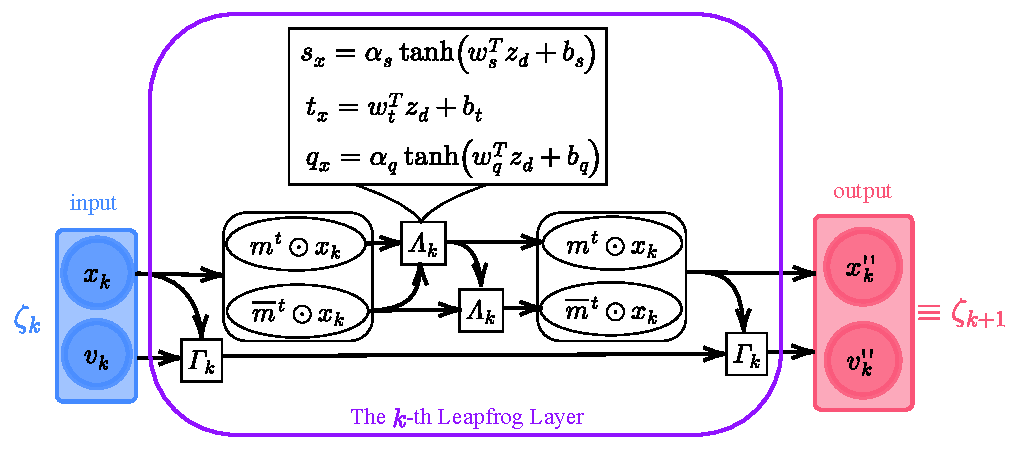
\includegraphics[width=\textwidth]{figures/network6.pdf}
   \caption{\label{fig:network}Illustration of the network architecture used in the \(x\) update, \Eqref{eq:new_position_update}.}
\end{figure}

Using this notation, we can write the complete leapfrog update (in the forward \(d=+1\) direction)\footnote{%
   To obtain the expression for the reverse direction, we can invert each of the
   \(\Gamma^{-}\equiv{\left(\Gamma^{+}\right)}^{-1}, \Lambda^{-}\equiv{\left(\Lambda^{+}\right)}^{-1}\) functions, and
   perform the updates in the opposite order.
} as:
%
\begin{enumerate}
   \item Half-step momentum update:%
      \hspace{29pt}\(%
         v^{\prime}_{k} = \Gamma^{+}_{k}(v_{k};\zeta_{v_{k}})%
   \)
   \item Full-step half-position update:\footnote{%
         By this we mean we are performing a complete update on one-half of the indices of \(x\) (determined by
         \(\mt\odot x\)), followed by an analogous update of the complementary indices, \(\mbart\odot x\).
   }
      \hspace{14pt} \(%
         x^{\prime}_{k} = \mbart\odot x_{k} + \mt\odot \Lambda^{+}_{k}(x_{k};\zeta_{x_{k}})
   \)
   \item Full-step half-position update:%
      \hspace{21pt} \(%
         x^{\prime\prime}_{k} = \mbart\odot\Lambda^{+}_{k}(x^{\prime}_{k};\zeta_{x^{\prime}_{k}}) + \mt\odot x^{\prime}_{k}
   \)
   \item Half-step momentum update:%
      \hspace{25pt} \(%
         v^{\prime\prime}_{k} = \Gamma_{k}^{+}(v^{\prime}_{k}; \zeta_{v^{\prime}_{k}})
   \)
\end{enumerate}
%
Collectively, we refer to this series of updates as a single \emph{leapfrog layer}, which performs a single update \(\xi\rightarrow\xi^{\prime}\).
%
Note that in order to keep our update reversible, we've split the \(x\) update into two sub-updates by
introducing a binary mask \(\mbart = \mathbbm{1} - \mt\) that updates half of the components of \(x\) sequentially.
%

As in HMC, we form a complete trajectory by performing \(N_{\mathrm{LF}}\) leapfrog steps in sequence, followed by a Metropolis-Hastings accept/reject step as described in \Eqref{eq:mhcriteria}.
%
However, unlike in the expression for HMC, we must take into account the overall Jacobian factor from the update
\(\xi\rightarrow\xi^{\prime}\), which can be easily computed as \(\left|\tfrac{\partial v^{\prime\prime}_{k}}{\partial
   v_{k}}\right| = \exp{\left(\tfrac{1}{2}{\varepsilon^{k}_{v}\cdot s^{k}_{v}(\zeta_{v_{k}})}\right)}\),
   \(\left|\tfrac{\partial x^{\prime\prime}_{k}}{\partial x_{k}}\right| = \exp{\left(\varepsilon^{k}_{x}\cdot s^{k}_{x}(\zeta_{x_{k}})\right)}\).
%
%
%%%%%%%%%%%%%%%%%%%%%%%%%%%%%%%%%%%%%%%%%%%%%%%%%%%%%%%%%%%%%%%%
\section{\label{sec:lattice_gauge_theory}Lattice Gauge Theory}
%
Let \(U_{\mu}(n) = e^{i x_{\mu}(n)} \in U(1)\), with \(x_{\mu}(n) \in [-\pi,\pi]\) denote the \emph{link
variables}, where \(x_{\mu}(n)\) is the link oriented in the \(\hat{\mu}\)-direction located at the site
\(n\).
%
We can write our target distribution in terms of the Wilson action \(S_{\beta}(x)\) as
%
\begin{equation}
   p_{t}(x) = e^{-\gamma_{t}\cdot S_{\beta}(x)},\quad\text{with}\quad S_{\beta}(x) = \beta\cdot \sum_{P}1 - \cos(x_{P})
   \label{eq:wilsonaction}
\end{equation}
%
where (\(1\).) \(\gamma_{t}\) is a scaling factor (\(\|\gamma_{t}\|<1\)) that is slowly annealed during training (\Secref{sec:annealing}) and (\(2\).) \(x_{P} \equiv x_{\mu}(n) + x_{\nu}(n+\hat{\mu}) - x_{\mu}(n+\hat{\nu}) -x_{\nu}(n)\) is the sum of the link
variables around the \(1\times1\) elementary plaquette, shown in \Figref{fig:plaquette}.
%
Here, \(\beta = 2 / g_{0}^{2}\) is a coupling constant and \(\beta\rightarrow\infty\) recovers the continuum limit of the theory. 
%

Physically, each lattice configuration can be characterized by its topological charge, \(\mathcal{Q}_{\mathbb{Z}}\in\mathbb{Z}\), defined as
%
\begin{equation}
      \mathcal{Q}_{\mathbb{Z}}(x) \equiv \frac{1}{2\pi}\sum_{P}\left\lfloor x_{P}\right\rfloor,
   \quad\text{where}\quad \left\lfloor x_{P}\right\rfloor = x_{P} -
   2\pi\left\lfloor\frac{x_{P}+\pi}{2\pi}\right\rfloor.
   \label{eq:intcharge}
\end{equation}
%
Current methods are severely limited in their ability to mix between different topologies, a phenomenon known as topological freezing.
%
For this reason, we wish to construct a loss function that encourages our sampler to explore different topological sectors.
%
In order to do so, we introduce a continuous version of the topological charge, \(\mathcal{Q}_{\mathbb{R}}\in\mathbb{R}\) by replacing the projection in \Eqref{eq:intcharge} as:
%
\begin{equation}
    \mathcal{Q}_{\mathbb{R}} \equiv \frac{1}{2\pi}\sum_{P}\sin(x_{P}).
    \label{eq:sincharge}
\end{equation}
%
This quantity has the advantage of being real-valued to help prevent numerical instability during training.
%
Our loss function is then defined as
%
\begin{equation}
   \mathcal{L}(\theta) = \mathbb{E}_{p(\xi)}{%
      \left[-\tfrac{1}{\ell^{2}}\cdot\delta(\xi^{\prime}, \xi)\cdot A(\xi^{\prime}|\xi)\right]
   }
\end{equation}
%
where \(\delta(\xi^{\prime}, \xi) \equiv {\left(\mathcal{Q}_{\mathbb{R}}(x^{\prime}) - \mathcal{Q}_{\mathbb{R}}(x)\right)}^{2}\) and \(A(\xi^{\prime}|\xi)\) is given in \Eqref{eq:mhcriteria}.
%
%

\section{\label{sec:braindump}Brain dump}
%
Using the training procedure in \Secref{sec:algorithm} with the annealing schedule from \Secref{sec:annealing}, we are able to train our sampler for some fixed number of training steps and then run inference on the trained model.
%

During training we maintain a buffer of \(M=2048\) chains which are updated in parallel.
%

We evaluate the loss function and update our weights accordingly at the end of each trajectory prior to performing the Metropolis-Hastings accept/reject step.
%

During inference, we record the values of quantities of interest and compare them to the results obtained from running inference using generic HMC.
%

To measure the improvement of our model, we evaluate the integrated autocorrelation time of the topological charge which can be interpreted roughly as the number of trajectories needed before we can expect a change in the charge value.
%

We can see in \Figref{fig:autocorr_vs_beta}, that the trained model out performs generic HMC across a range of coupling constants \(\beta = 2, 3, \ldots, 7\).
%

To ensure the validity of our results, each trained run was compared to multiple HMC runs across a range of \(N_{\mathrm{LF}}\) and \(\varepsilon\) values.
%

By introducing the scaling \(N_{\mathrm{LF}}\cdot\tau_{\mathrm{int}}\) we more accurately capture the computational effort per step when comparing the two approaches.
%

We see in ~\Figref{fig:topological_freezing} that HMC remains stuck at a particular value for large sections of the simulation, whereas the trained sampler rapidly jumps between values.
%

In order to better understand the mechanism driving this improved behavior, we evaluate different quantities at intermediate leapfrog layers during the trajectory.
%

If we think of the average plaquette as being an energy density, we can see in \Figref{fig:plaqsf}, \Figref{fig:hwf} that our sampler experiences a gradual increase in energy during the first half of the trajectory before decreasing back to its original value at the end.
%
We believe that this ability to increase and decrease the energy within a trajectory helps the sampler to overcome energy barriers between topological sectors whereas HMC remains stuck.
%

%
\begin{figure}[htpb]
   \centering
   \begin{subfigure}{0.34\textwidth}
      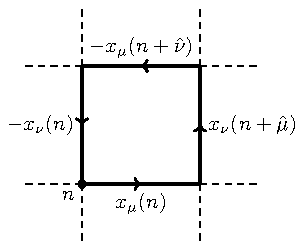
\includegraphics[width=\textwidth]{figures/plaq_tikz.pdf}
      \caption{\label{fig:plaquette}Plaquette, \(P\)}
   \end{subfigure}
   %
   \hfill
   %
   \begin{subfigure}{0.65\textwidth}
      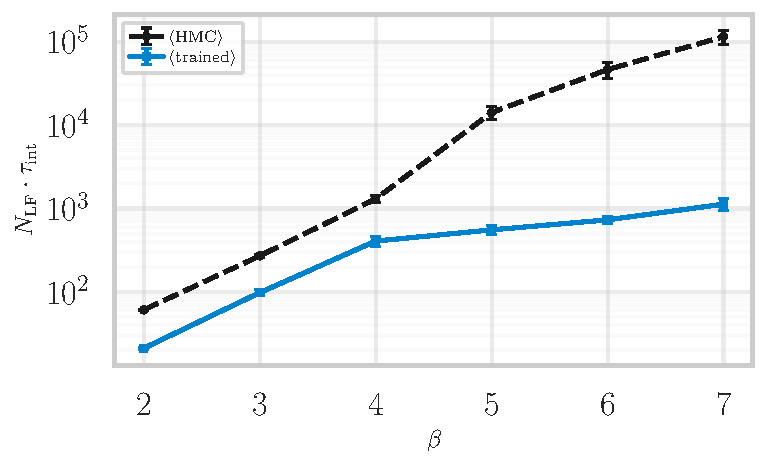
\includegraphics[width=\textwidth]{figures/autocorr_vs_beta_blue_2120.pdf}
      \caption{\label{fig:autocorr_vs_beta}Estimate of the integrated autocorrelation time
      \(\tau_{\mathrm{int}}^{\mathcal{Q}_{\mathbb{R}}}\) vs \(\beta\), scaled by \(N_{\mathrm{LF}}\) to account for
   different trajectory lengths.}
         % for HMC (black dashed line), trained model (solid blue line).}
   \end{subfigure}
   \hfill
   %
   \begin{subfigure}{\textwidth}
      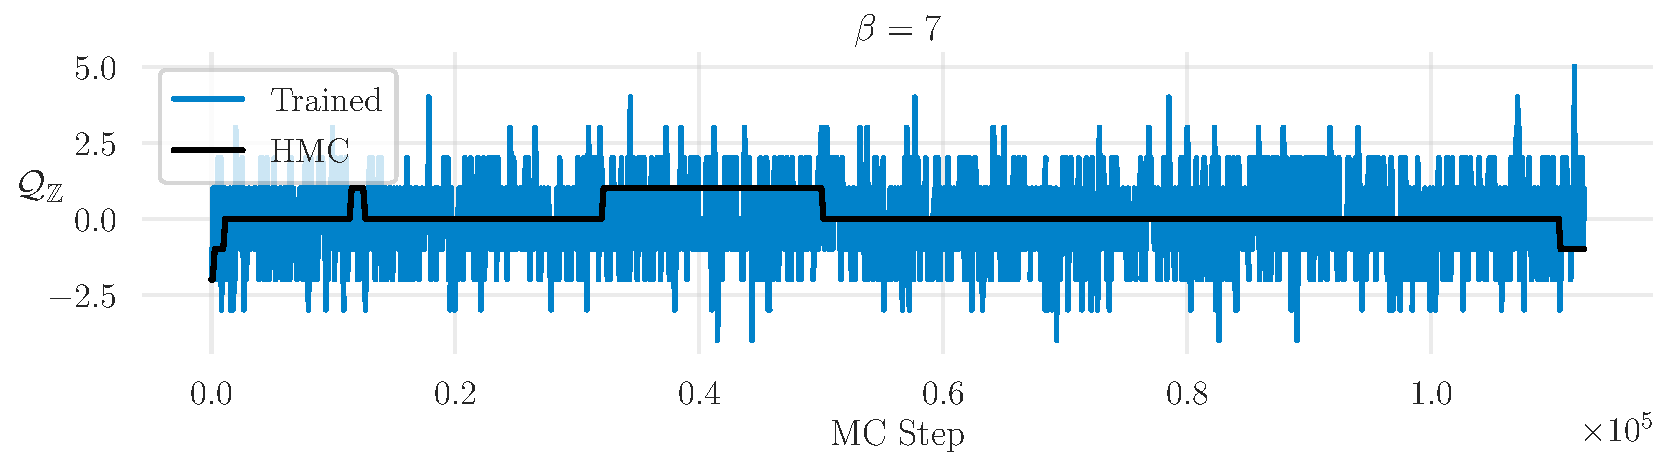
\includegraphics[width=\textwidth]{figures/topological_freezing_anl_blue_wide.pdf}
      \caption{\label{fig:topological_freezing}Topological charge \(\mathcal{Q}_{\mathbb{R}}\) vs MC
      step for both HMC (black line) and the trained model (blue line).}% for HMC (black line), and trained model (blue line)}
   \end{subfigure}
   %
   \hfill
   %
   \begin{subfigure}{0.31\textwidth}
      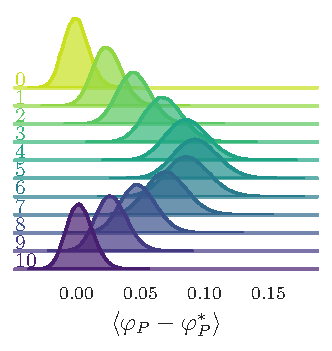
\includegraphics[width=\textwidth]{figures/plaqsf_1758.pdf}
      \caption{\label{fig:plaqsf}Change in the average plaquette, \(\langle x_{P}-x_{P}^{*}\rangle\) at intermediate leapfrog layers.}
   \end{subfigure}
   \hfill
   \begin{subfigure}{0.31\textwidth}
      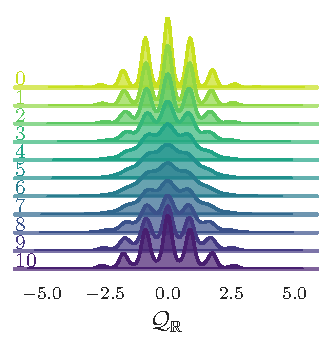
\includegraphics[width=\textwidth]{figures/sinQf_1755.pdf}
      \caption{\label{fig:sinQf}The real-valued topological charge, \(\mathcal{Q}_{\mathbb{R}}\) at intermediate leapfrog layers.}%
   \end{subfigure}
   %
   \hfill
   \begin{subfigure}{0.31\textwidth}
      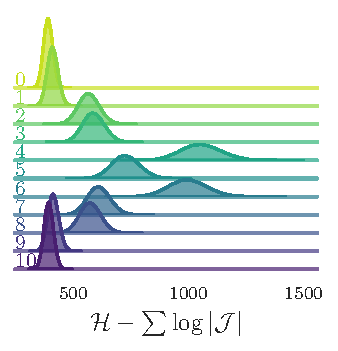
\includegraphics[width=\textwidth]{figures/extras/hwf.pdf}
      \caption{\label{fig:hwf}The readjusted energy, \(\mathcal{H}-\sum\log|\mathcal{J}|\), of the model at intermediate leapfrog layers.}
   \end{subfigure}
\end{figure}
%

\subsubsection*{Acknowledgments}
This research was performed on ThetaGPU using resources of the Argonne Leadership Computing Facility (ALCF), which is a DOE office of science user
facility supported under contract DE\_AC02--06CH11357.%
%
This work describes objective technical results and analysis.
%
Any subjective views or opinions that might be expressed in the work do not necessarily represent the views of the u.s.
doe or the united states government.

\bibliography{iclr2021_conference}
\bibliographystyle{iclr2021_conference}

\appendix
\section{Appendix}
%
\subsection{\label{subsec:HMC}Hamiltonian Monte Carlo (HMC)}
%
The Hamiltonian Monte Carlo algorithm is a widely used technique that allows us to sample from an analytically known
target distribution \(p(x)\) by constructing a chain of states \(\{x^{(0)}, x^{(1)}, \ldots, x^{(n)}\}\), such that
\(x^{(n)}\sim p(x)\) in the limit \(n\rightarrow\infty\).
%
For our purposes, we assume that our target distribution can be expressed as a Boltzmann distribution, \(p(x) =
\tfrac{1}{\mathcal{Z}} e^{-S(x)}\propto e^{-S(x)}\), where \(S(x)\) is the \emph{action} of our theory, and
\(\mathcal{Z}\) is a normalization factor (the partition function).
%
In this case, HMC begins by augmenting the state space with a fictitious momentum variable \(v\), normally
distributed independently of \(x\), i.e.\ \(v\sim\mathcal{N}(0, \mathbbm{1})\).
%
Our joint distribution can then be written as \(%
   p(x, v) = p(x)\cdot p(v) \propto e^{-S(x)}\cdot e^{-\frac{1}{2}v^{T}v} = e^{-\mathcal{H}(x, v)}
\), where \(\mathcal{H}(x, v)\) is the Hamiltonian of the joint (x, v) system.
%
This system obeys Hamilton's equations: % 
\(\dot{x} = \frac{\partial\mathcal{H}}{\partial v}\), \(\dot{v} = -\frac{\partial H}{\partial x}\), which can be 
numerically integrated using the leapfrog integrator along iso-probability contours of \(\mathcal{H} = \text{const.}\).
%
Explicitly, for a step size \(\varepsilon\) and initial state \(\xi = (x, v)\), the leapfrog integrator generates a
proposal configuration \(\xi^{\prime} \equiv (x^{\prime}, v^{\prime})\) by performing the following series of updates: 
%
\subsection{\label{subsec:leapfroghmc}Leapfrog Update}
%
\begin{enumerate}
   \item Half-step momentum update: \hspace{12pt}\(%
      v^{1/2} \equiv v{\left(t+\frac{\varepsilon}{2}\right)} = v-\frac{\varepsilon}{2}\partial_{x}S(x)
   \)
   \item Full-step position update: \hspace{36pt}\(%
      x^{\prime} \equiv x(t+\varepsilon) = x + \varepsilon v^{1/2}
   \)
   \item Half-step momentum update:
      \hspace{18pt} \(%
         v^{\prime} \equiv v(t+\varepsilon) = v^{1/2} - \frac{\varepsilon}{2}\partial_{x} S(x^{\prime})
   \)
\end{enumerate}
%
We can then construct a complete \emph{trajectory} of length \(\lambda = \varepsilon\cdot N_{\mathrm{LF}}\) by
performing \(N_{\mathrm{LF}}\) leapfrog steps in sequence.
%
At the end of our trajectory, we either accept or reject the proposal configuration according to the Metropolis-Hastings
acceptance criteria,
%
\begin{equation}
   x_{i+1} =
   \begin{cases}%
      x^{\prime} &\mbox{with probability } A(\xi^{\prime}|\xi) \\
      x &\mbox{with probability } (1 - A(\xi^{\prime}|\xi)), \quad\text{and}\quad%
         A(\xi^{\prime}|\xi) = \min\left\{%
            1, \frac{p(\xi^{\prime})}{p(\xi)}\left|\frac{\partial{\xi^{\prime}}}{\partial\xi^{T}}\right|%
         \right\}.
   \end{cases}
   \label{eq:mhcriteria}
\end{equation}
%
The generic leapfrog integrator is known to be symplectic (conserves energy), so the Jacobian factor reduces to
\(\left|\frac{\partial\xi^{\prime}}{\partial\xi^{T}}\right| = 1\). 
%
\section{\label{sec:annealing}Annealing Schedule}
%
To help our sampler overcome the large energy barriers between isolated modes, we introduce an \emph{annealing schedule}
during the training phase (\(N\) training steps) \({\{\gamma_{t}\}}_{t=0}^{N} = \{\gamma_{0}, \gamma_{1}, \ldots,
\gamma_{N-1}, \gamma_{N}\}\), where \(\gamma_{0} < \gamma_{1} < \cdots < \gamma_{N} \equiv 1\), \(\gamma_{t+1} -
\gamma_{t} \ll 1\).
%
Note that we are free to vary \(\gamma\) during the initial training phase as long as we recover the true distribution
with \(\gamma \equiv 1\) at the end of training and evaluate our trained model without this factor.
%
Explicitly, for \(\gamma_{t} < 1\) this rescaling factor helps to reduce the height of the energy barriers, making it
easier for our sampler to explore previously inaccessible regions of the phase space.
%
In terms of this additional annealing schedule, our target distribution picks up an additional index \(t\) to represent
our progress through the training phase, which can be written explicitly as 
%
\begin{equation}
   p_{t}(x)\propto e^{-\gamma_{t} S(x)},\quad\text{for}\quad t=0, 1, \ldots, N
   \label{eq:targetannealing}
\end{equation}
%
\section{\label{sec:algorithm}Training Algorithm}
%
\begin{algorithm}[htpb]%
   \SetAlgoLined%
   \SetAlgoVlined%
   \SetKwProg{Fn}{def}{\string:}{}%
   \SetKwFunction{Range}{range}%
   \SetKwFor{For}{\color{blue}\textbf{\texttt{for}}}{\string:}{}\color{black}%
   \SetKwIF{If}{ElseIf}{Else}{if}{:}{elif}{else:}{}%
   \SetKwFor{While}{while}{:}{fintq}%
   \SetKwInOut{Input}{\color{red}{\textbf{\texttt{input}}}\color{black}}%
   \SetKwInOut{Output}{\color{red}{\textbf{\texttt{output}}}\color{black}}%
   \AlgoDontDisplayBlockMarkers\SetAlgoNoEnd%
   \DontPrintSemicolon%
   \caption{\label{alg:training_algorithm}Training procedure}%
   \Input{%
         %(1.) \texttt{Target distribution,} \(p_{t}(x)\propto e^{-\beta_{t} U(x)}\)
         %(2.) \texttt{Loss function}, \(\mathcal{L}_{\theta}(\xi^{\prime},\xi,
         %   A (\xi^{\prime}|\xi))\)
         %(3.) \texttt{Learning rate schedule}, \({\{\alpha_{t}\}}_{t=0}^{N_{\mathrm{train}}}\)
         %(4.) \texttt{Annealing schedule}, \({\{\gamma_{t}\}}_{t=0}^{N_{\mathrm{train}}}\)
         %(5.) \texttt{Batch of initial states}, \(x\)
      % {}\\
      \begin{enumerate}
         \item \texttt{Target distribution,} \(p_{t}(x)\propto e^{-\beta_{t} U(x)}\)
         \item \texttt{Loss function}, \(\mathcal{L}_{\theta}(\xi^{\prime},\xi,
            A(\xi^{\prime}|\xi))\)
         \item \texttt{Learning rate schedule}, \({\{\alpha_{t}\}}_{t=0}^{N_{\mathrm{train}}}\)
         \item \texttt{Annealing schedule}, \({\{\gamma_{t}\}}_{t=0}^{N_{\mathrm{train}}}\)
         \item \texttt{Batch of initial states}, \(x\)
      \end{enumerate}
   }%
   \texttt{Initialize weights} \(\theta\)\;
   % {}\;
   \For{\(0 \leq t < N_{\mathrm{train}}\)}{%
      % {}\;
      \texttt{update:} \(p_{t}(x)\propto e^{-\beta_{t}U(x)}\)\;
      \texttt{resample:} \(v\sim\mathcal{N}(0, \mathbbm{1})\)\;
      \texttt{resample:} \(d\sim\mathcal{U}(+,-)\)\;
      \texttt{construct:} \(\xi \equiv (x, v, d)\)\;
      % {}\;
      \For{\(0 \leq \ell < N_{\mathrm{LF}}\)}{%
         \texttt{propose:} \(\xi_{\ell}^{\prime}\leftarrow\mathbf{FL}_{\ell}^{\pm}\xi_{\ell}\)
      }
      \texttt{compute:} \(A(\xi^{\prime}|\xi) =%
      \min\left\{1,\frac{p(\xi^{\prime})}{p(\xi)}\left|\frac{\partial%
      \xi^{\prime}}{\partial \xi^{T}}\right|\right\}\)\;
      % {}\;
      \texttt{update:} \(\mathcal{L}\leftarrow \mathcal{L}_{\theta}(\xi^{\prime},\xi,%
      A(\xi^{\prime}|\xi))\)\;
      % {}\;
      \texttt{backprop:} \(\theta\ \leftarrow\ \theta-\alpha_t \nabla_{\theta} \mathcal{L}\)\;
      % {}\;
      \texttt{assign:} \(x_{t+1} \leftarrow
      \begin{cases}
         x^{\prime} &\mbox{with probability } A(\xi^{\prime}|\xi) \\
         x &\mbox{with probability } (1 - A(\xi^{\prime}|\xi)).%
      \end{cases}%
      \)\;
   }\;
\end{algorithm}%
%
%\section{\label{sec:hyperparameters}Hyperparameters}
%\begin{table}[]
%\begin{tabular}{|l|l|l|l|l|l|l|l|l|l|}
%\hline
% & \(N_{\mathrm{LF}}\) & \(\beta_{0}\) & \(\beta_{1}\) & train steps & hidden layer sizes & activation function & dropout probability & batch norm layer &  \\ \hline
%1 &  &  &  &  &  &  &  &  &  \\ \hline
%  &  &  &  &  &  &  &  &  &  \\ \hline
%  &  &  &  &  &  &  &  &  &  \\ \hline
%  &  &  &  &  &  &  &  &  &  \\ \hline
%  &  &  &  &  &  &  &  &  &  \\ \hline
%  &  &  &  &  &  &  &  &  &  \\ \hline
%  &  &  &  &  &  &  &  &  &  \\ \hline
%\end{tabular}
%\end{table}
%
\end{document}